\section{The Live Research Manager}
\label{sec:live-pm}

The previous section defines the \ara{} protocol: a structured target format for research knowledge.
A natural question follows: \emph{who populates it?}
Requiring researchers to hand-author structured files would simply replace one documentation burden with another, negating the very tax the protocol was designed to eliminate.

The key observation is that in AI-native research, the full research trajectory---every design choice, failed experiment, and hard-won heuristic---already exists as machine-readable text in the conversation between researcher and agent.
The Live Research Manager crystallizes this latent signal into a living \ara{} artifact that accumulates organically in the background, with zero documentation overhead for the researcher.\footnote{\url{github.com/AmberLJC/Agent-Native-Research-Artifact}}
We derive design principles from the AI-native paradigm (\S\ref{sec:design-principles}) and present the system that realizes them (\S\ref{sec:lrm-design}; Figure~\ref{fig:lrm-overview}).

\begin{figure}[t!]
\centering
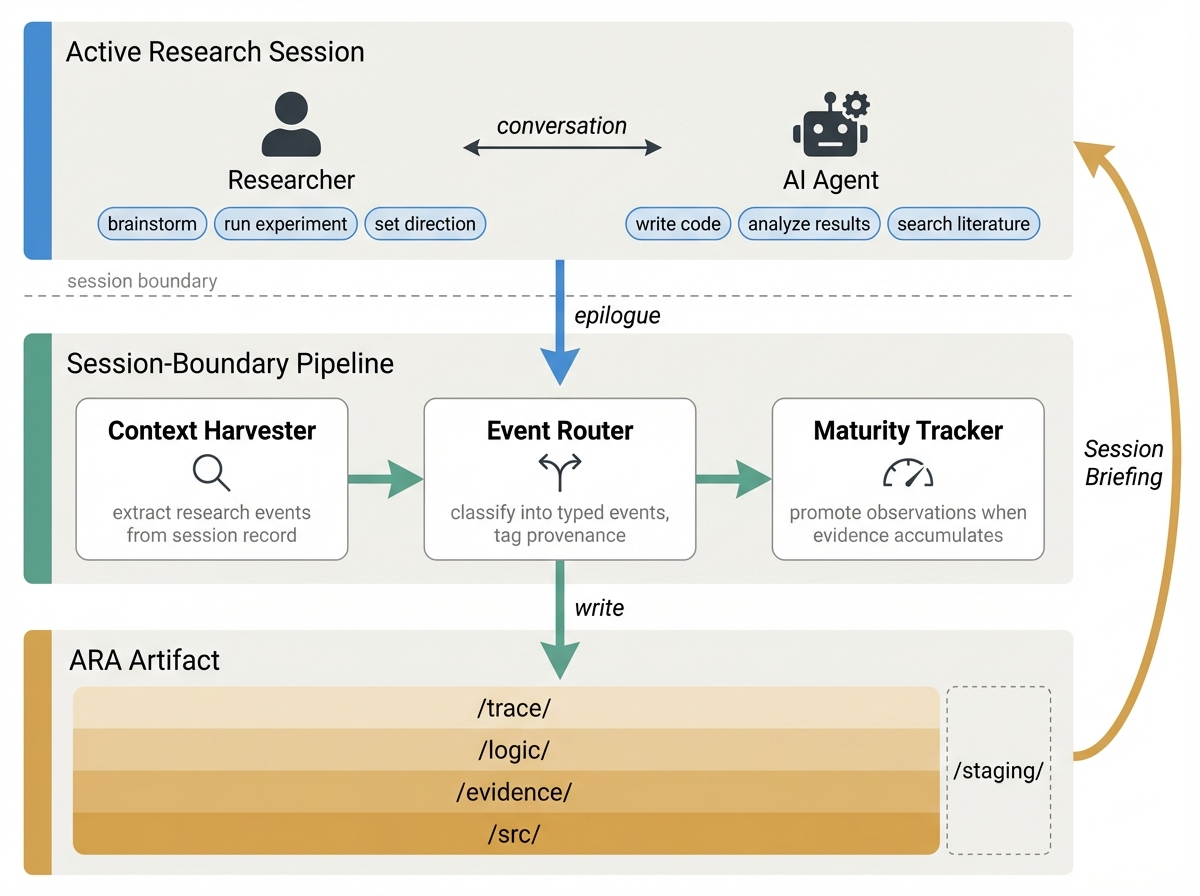
\includegraphics[width=\linewidth]{figures/fig_lrm_lifecycle_v5_attempt2.png}
\caption{The Live Research Manager operates at session boundaries: a three-stage pipeline (Context Harvester $\to$ Event Router $\to$ Maturity Tracker) distills each researcher--agent conversation into typed events that accumulate across \ara{} layers over time.}
\label{fig:lrm-overview}
\end{figure}

\subsection{Design Principles}
\label{sec:design-principles}

\paragraph{AI-native research.}
Computer science research is increasingly \emph{AI-native}: the researcher collaborates with a general-purpose coding agent across the full research lifecycle.
A single conversational loop may span brainstorming a hypothesis, surveying related work, writing and debugging experiment code, analyzing results, and drafting the paper---the researcher provides direction, the agent executes, and the cycle repeats across days or weeks.
This paradigm shift has a structural consequence: for the first time, the research process is \emph{born digital and born textual}.
Every instruction, intermediate result, design choice, and abandoned direction already exists as machine-readable text---the raw material for a complete research record, lacking only a system to let it crystallize naturally.
Prior efforts to preserve process knowledge---negative-result journals~\citep{matosin2014negativity}, registered reports~\citep{chambers2013registered}---foundered because documentation remained a separate, unrewarded burden on the researcher.
AI-native research dissolves this barrier: the process trace is not an additional deliverable but a \emph{byproduct} of the research itself, generated automatically in every researcher--agent session.
We are, in other words, at the first moment in scientific history where comprehensive research-process capture is feasible at negligible marginal cost.

This observation motivates the Live Research Manager: if the research trajectory is already captured in conversation, a background system can distill it into a structured \ara{} without asking the researcher to document anything.
We derive three design principles from this paradigm.

\begin{enumerate}[label=\textbf{P\arabic*.}, leftmargin=2em, itemsep=1pt]
    \item \textbf{Silent, framework-independent integration}: the manager is a natural-language specification loadable by any coding agent, requiring no custom SDKs. It runs as a background process that silently collects research traces without researcher intervention.
    \item \textbf{Faithful epistemic provenance}: every event is tagged with provenance (\texttt{user}, \texttt{ai-suggested}, \texttt{ai-executed}, \texttt{user-revised}) to preserve epistemic origin. Raw observations are staged rather than forced into categories, maturing progressively into typed events as evidence accumulates, so downstream consumers can reconstruct not just \emph{what} was concluded but \emph{why}.
    \item \textbf{Comprehensive trajectory capture}: the full branching research process, including dead ends and pivots, is recorded with cross-layer bindings established at capture time. The artifact is version-controlled, so each milestone produces a navigable snapshot and retroactive revisions are first-class operations rather than destructive overwrites.
\end{enumerate}
\noindent Full rationale for each principle is in Appendix~\ref{app:lrm-principles}.

\subsection{System Design}
\label{sec:lrm-design}

\paragraph{Overview.}
We implement the Live Research Manager as an \emph{agent skill}~\cite{agentskills2025}: a lightweight, natural-language specification that, when loaded into a general-purpose coding agent's context window, turns it into a domain-specialized agent (\textbf{P1}).
A skill requires no custom SDKs or infrastructure; it simply composes tools the agent already possesses (file read, write, edit, shell execution) with domain knowledge of the \ara{} schema, and artifact quality improves automatically as the underlying language model advances.
The skill is open-source and available at \url{https://github.com/AmberLJC/Agent-Native-Research-Artifact}.

The manager remains silent during active research, then runs a three-stage retrospective pipeline at the end of each conversation (\textbf{P1}; Figure~\ref{fig:lrm-overview}).
The \textbf{Context Harvester} scans the session record---conversational history, tool outputs, experiment results, and code diffs---to extract research-significant events.
The \textbf{Event Router} classifies each event, tags it with provenance, and writes it to the appropriate \ara{} layer.
The \textbf{Maturity Tracker} reviews the staging area, promoting observations that have accumulated sufficient evidence into formal entries and flagging stale or conflicting items.
At the start of the next session, the manager reads the artifact back to surface a structured briefing, closing the loop.
The remainder of this subsection details each stage and the cross-session mechanisms that bind them together.
\paragraph{Context harvesting and event routing.}
The Context Harvester scans the full session record and identifies two categories of research-significant activity: actions the AI agent has already performed (e.g., experiment runs, code changes, literature searches) and directions the researcher has expressed or confirmed (e.g., hypotheses to test, design choices, abandoned approaches).
The Event Router then classifies each extracted event into one of seven types (Table~\ref{tab:event-types}) and tags it with provenance (\textbf{P2})---\texttt{user}, \texttt{ai-suggested}, \texttt{ai-executed}, or \texttt{user-revised}.
An \texttt{ai-suggested} event never auto-upgrades until the researcher explicitly confirms it, preserving the epistemic integrity of the artifact.
Event payloads follow the protocol's factual-density requirement (\S\ref{sec:philosophy}): conversational prose is distilled into telegraphic, quantitative language before committing to the artifact.
Each typed event is written to the appropriate \ara{} layer: trace events (decisions, experiments, dead ends, pivots) append to the Exploration Graph (\texttt{/trace/}), building a faithful, chronological record of the research trajectory including the directions that were tried and abandoned (\textbf{P3}); claims and heuristics enter the Cognitive Layer (\texttt{/logic/}); and events that resist classification are staged in \texttt{/staging/} for later promotion.

\begin{table*}[!t]
\centering
\small
\begin{tabular}{@{}ll@{\hskip 1.5em}ll@{}}
\toprule
\textbf{Event Type} & \textbf{Structured Payload} & \textbf{Event Type} & \textbf{Structured Payload} \\
\midrule
\texttt{decision}    & Choice, alternatives, evidence        &
\texttt{claim}       & Statement, falsification criteria     \\
\texttt{experiment}  & Metrics, claim linkage                &
\texttt{heuristic}   & Trick, sensitivity, bounds            \\
\texttt{dead\_end}   & Hypothesis, failure mode, lesson      &
\texttt{observation} & Raw finding, awaiting classification  \\
\texttt{pivot}       & Trigger, rationale                    &
& \\
\bottomrule
\end{tabular}
\caption{Research event types and structured payloads.}
\label{tab:event-types}
\vspace{-4pt}
\end{table*}

\paragraph{Progressive crystallization.}
Artifact construction proceeds at two timescales (\textbf{P2}).
\emph{Continuously}, at every session boundary, the manager appends trace events to the Exploration Graph, recording how the researcher navigates the open-ended research landscape.
\emph{Periodically}, when a major milestone is reached---a hypothesis confirmed or refuted, a working prototype completed, a key design choice finalized---the Maturity Tracker \emph{crystallizes} the accumulated observations into the more structured layers of the artifact.
Raw observations mature into formal claims in the Cognitive Layer (\texttt{/logic/}), working code is documented in the Physical Layer (\texttt{/src/}), and concepts are added to the knowledge index.
This two-phase rhythm mirrors how research understanding actually develops: insights begin as scattered observations, and forcing premature structure would distort the record.
The manager stages what is not yet classifiable and crystallizes only when \emph{closure signals} in the session record---topic abandonment, explicit researcher affirmation, empirical resolution of linked experiments, or artifact-level commitment---indicate the observation has been treated as settled (Appendix~\ref{app:lrm-maturity}).
When a pivot invalidates an earlier design choice, the manager propagates the change: it updates the affected artifact entries (claims, heuristics, or configuration) to reflect the new direction while the Exploration Graph retains the original rationale and the reason for revision.
Because the artifact is version-controlled, each milestone crystallization produces a commit, giving the project a navigable history of its intellectual evolution, much as GitHub provides for code.

\paragraph{Cross-session continuity.}
The manager is stateless; the artifact itself carries memory across sessions. At session close, it writes a short session record (events captured, claims touched, open threads) and appends to a running session index. The next session reads this index alongside the current claims and staged observations, and raises the relevant pieces only when they bear on the task at hand, rather than leading with a formal briefing the researcher did not ask for (Appendix~\ref{app:lrm-continuity}).
